% Created 2014-04-14 Mon 18:10
\documentclass[runningheads,a4paper]{llncs}
\usepackage[utf8]{inputenc}
\usepackage[T1]{fontenc}
\usepackage{fixltx2e}
\usepackage{graphicx}
\usepackage{float}
\usepackage{wrapfig}
\usepackage{amsmath}
\usepackage{textcomp}
\usepackage{marvosym}
\usepackage{wasysym}
\usepackage{amssymb}
\usepackage{hyperref}
\usepackage{microtype}
\usepackage{acronym}
\tolerance=1000
\usepackage[usenames,dvipsnames]{xcolor}
\usepackage{listings}

\urldef{\mailsa}\path|{joel.kuiper, m.a.swertz}@rug.nl|
\urldef{\mailsb}\path|iain.marshall@kcl.ac.uk|
\urldef{\mailsc}\path|byron_wallace@brown.edu|

\acrodef{ebm}[EBM]{Evidence-based Medicine}

\institute{
  University of Groningen P.O. Box 30001, 9700 RB Groningen \\ \mailsa
  \and King's College London, London SE1 3QD, UK \\ \mailsb
  \and Brown University, Providence, RI 02906, USA \\ \mailsc}

\begin{document}
\setcounter{tocdepth}{3}
\newcommand{\highlight}[1]{\colorbox{yellow}{#1}}

% Autogenerated, do not edit
\newcommand{\revisiondate}{2014-04-24}
<<<<<<< HEAD
\newcommand{\revision}{3f2c73a}
=======
\newcommand{\revision}{d58899a}
>>>>>>> 1b257ee... updates

\author{Kuiper, J\inst{1}. \and Marshall, I.J.\inst{2} \and Wallace, B.C.\inst{3} \and Swertz, M.A.\inst{1}}
\date{\today}
\title{Spá: a web-based viewer for text mining in Evidence Based Medicine}


\maketitle
\begin{abstract}
Unstructured PDF documents remain the main vehicle for dissemination of scientific findings.
Those interested in gathering and assimilating data must therefore manually peruse published articles and extract from these the elements of interest.
\acl{ebm} provides a compelling illustration of this: many person-hours are spent each year extracting summary information from articles that describe clinical trials.
Machine learning provides a potential means of mitigating this burden by automating extraction.
But, for automated approaches to be useful to end-users, we need tools that allow domain experts to interact with, and benefit from, model predictions.
To this end, we present an web-based tool called Spá\footnote{available under GPLv3 at \url{https://github.com/joelkuiper/spa} \cite{kuiper2014}} that accepts as input an article and provides as output an automatically visually annotated rendering of this article.
More generally, Spá provides a framework for visualizing predictions, both at the document and sentence level, for full-text PDFs.
\\
\\
\texttt{revision: \revision, date: \revisiondate}
\end{abstract}

\acresetall

\section{Introduction}
\label{section:intro}
Finding sentences or words with particular characteristics within a document is an important task in natural language processing and machine learning.

Consider \ac{ebm} \cite{sackett1996}, which addresses clinical questions by identifying and synthesizing data from all relevant published articles.
When doing this one needs, for example, to assess the \emph{risk of bias} for a particular study across different domains, like bias due to improper blinding of participants and personnel.
For this task, one wants to make a summary judgement (e.g., low risk of bias) and simultaneously extract the sentences supporting that judgement.

Extracting such information from the unstructured text of clinical trial articles is a laborious process.
Machine learning methods provide the machinery to automate such extractions; as they can effectively impose structures onto PDF's.
But if such technologies are to be practically useful, we need tools to visualize the predictions.
Here we describe Spá which aspires to realize this aim.
Spá is an open-source, web-based tool that can incorporate state-of-the-art machine learning predictors to automatically annotate PDF articles.
Furthermore we have created machine learning systems on describing clinical trials with risk of bias predictions and extracted sample sizes.
This tool is useful for practitioners of \ac{ebm} and other biomedical researchers.

\begin{figure}[htb]
\centering
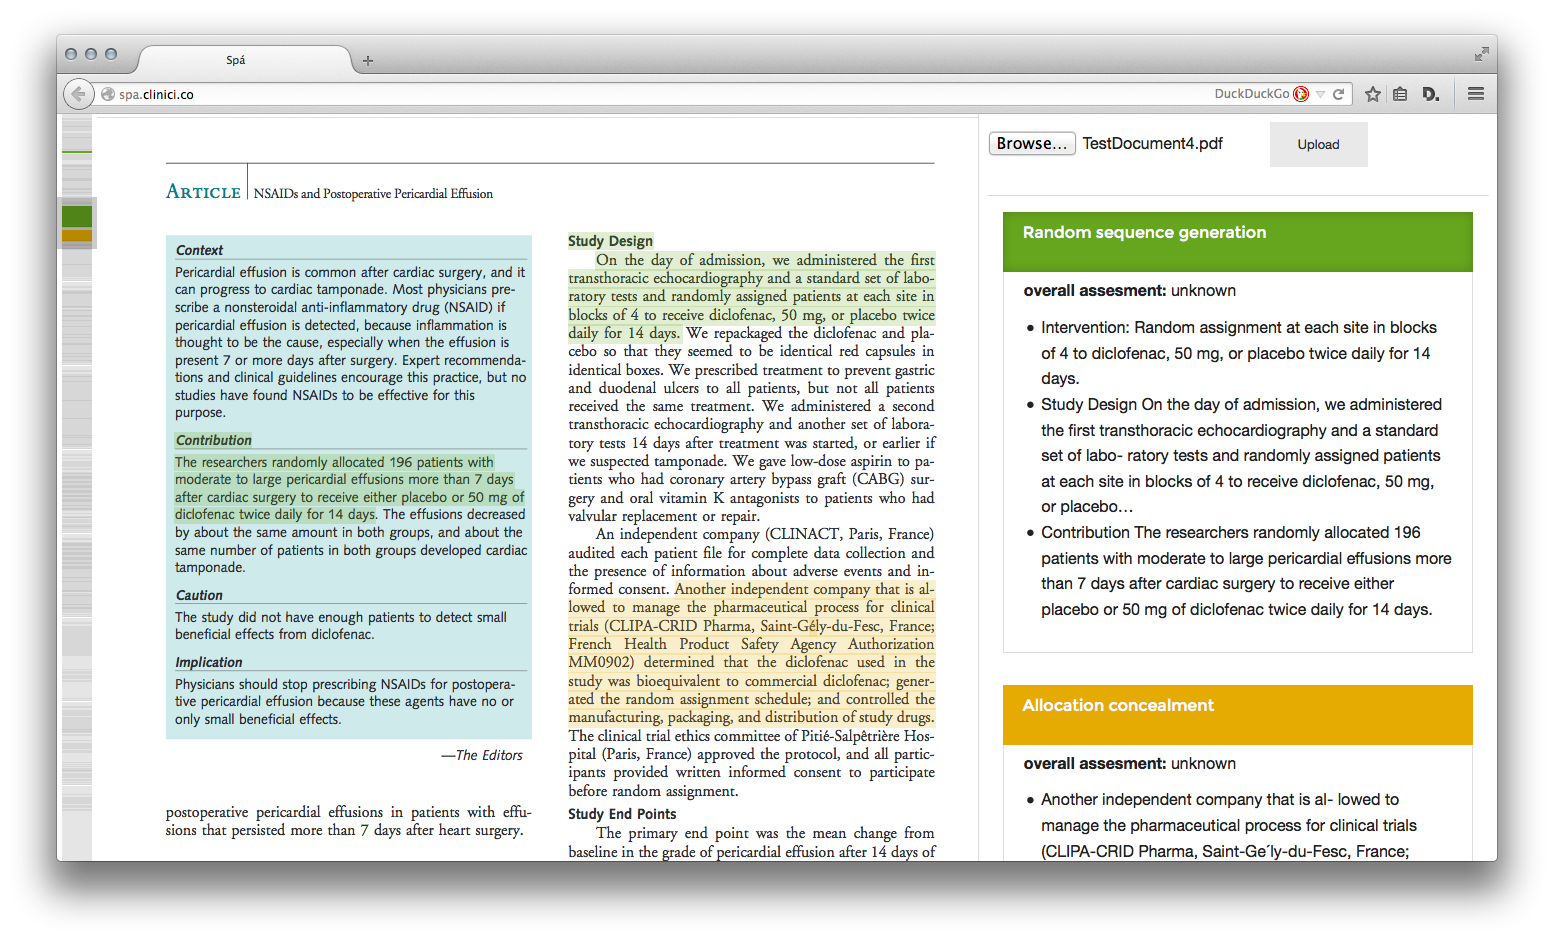
\includegraphics[width=.9\linewidth]{./images/screenshot.png}
\caption{\label{fig:screensot}Screenshot of a PDF with highlighted risk of bias}
\end{figure}

While our application of interest is \ac{ebm}, we emphasize that the tool can be used in any domain.
Thus the contribution of this work is two-fold, as we present:
(1) a practical tool that incorporates machine learning to help researchers rapidly assess published medical articles, and,
(2) a general open-source web tool for visualizing the predictions of trained models from full-text articles.
These contributions are described further in sections \ref{section:EBM-ML} and \ref{section:architecture}, respectively.

\section{Automating \acl{ebm}}
\label{section:EBM-ML}

\subsection{Systematic Reviews}
The process of pooling and summarizing clinical trials is called \emph{systematic reviewing}, and forms the corner-stone of current \ac{ebm}.
Systematic reviewing consists of specifying an inclusion criteria, searching the literature, screening the retrieved citations to identify eligible studies and, finally, summarizing the relevant evidence.
But achieving this aim is complicated by the massive numbers of trials that are conducted: for example, the Cochrane Library alone indexes 286,418 trials as having been conducted in the last decade \cite{valkenhoef2012}.
While methods and publishing standards are improving, a lot of legacy publications will remain only as PDF documents.

To aid the process of systematic reviewing we made a web-based tool that allows the visualization of annotations within a PDF documents, and meta-information alongside it.

\subsection{Machine Learning Strategies}
When doing risk of bias assessment one wishes to \highlight{todo}

% \begin{itemize}
% \item Basically show that we're using state of the art
% \item Briefly talk about cochrane DB / distant supervision
% \item KDD stuff (briefly)
% \item Multi-task stuff!
% \end{itemize}

\section{Architecture overview}
\label{section:architecture}
\begin{figure}[htb]
\centering
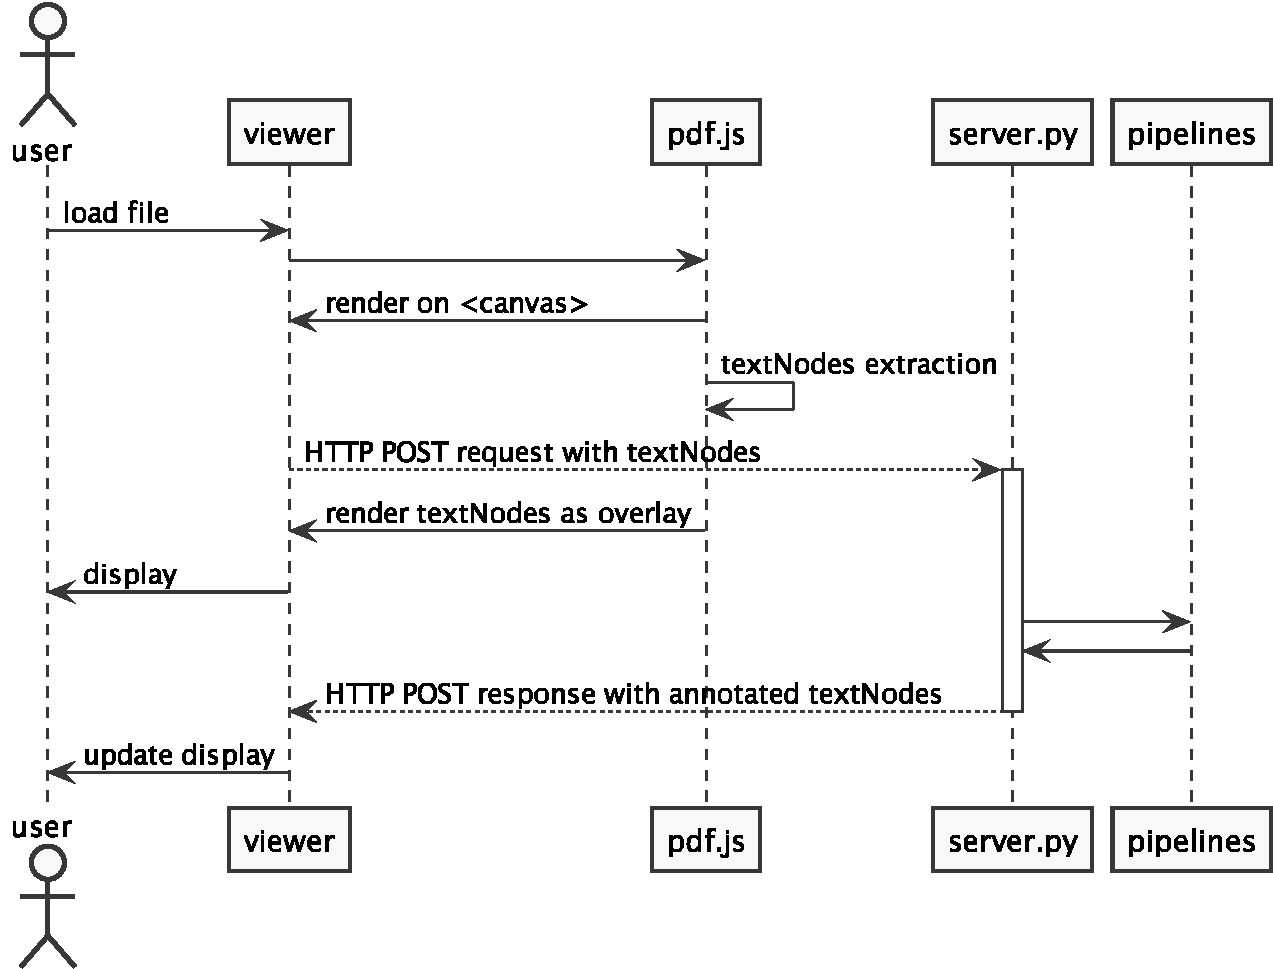
\includegraphics[width=.9\linewidth]{./diagrams/sequence.pdf}
\caption{\label{fig:sequence}Sequence diagram of a typical request-response}
\end{figure}
Spá relies on Mozilla pdf.js\footnote{\url{http://mozilla.github.io/pdf.js}} for visualization of the document and text extraction.
The results of the text extraction are processed server-side by a variety of processing topologies, as outlined in figure \ref{fig:sequence}.
Results, which could come from complicated machine learning systems, are communicated back to the browser and displayed using React components\footnote{\url{http://facebook.github.io/react}}.

For each of the annotations the relevant nodes in the document are highlighted and a custom scrollbar, inspired by \href{http://substance.io/}{substance.io}, that acts as a mini-map is projected to show where it resides within the document.
The user can interactively activate and inspect specific results.

\section{Conclusion \& Future work}
We present a web-based tool for interactive visualization of annotations and meta-data on PDF documents.
This allows users to see the results from machine learning systems within the context of a specific document.
Moreover, we present a case study for \ac{ebm} by automatically extracting potential Risks of Bias, with supporting sentences.

However, we believe the tool to be useful for a much wider range of text mining and machine learning applications.
To increase the generality of the tool work is being done to support a pluggable system for processing topologies, allowing developers to quickly plug in new systems.
Furthermore, work is being done on allowing users to save selected annotations, possibly embedded within the document itself, for sharing and off-line use.
The ultimate vision is to have a extensible system for semi-automated (machine assisted) screening, data extraction and data summarization.

\subsubsection{Acknowledgments}
Part of this research was funded by the European Union Seventh Framework Programme (FP7/2007-2013) under grant agreement n° 261433

\bibliographystyle{splncs}
\bibliography{references}

\end{document}
